%%%%
% -- Instrument Description
% --     FOBOS Keck White Paper 2019
%%%%


\section{FOBOS Instrument Description}
\label{sec:concept}
% \noindent \comment{1 page}

% Here's an alternative way to put in figures if we want captions on the side (to save space)
% Could introduce a new ``counter'' to count and label figures appropriately
%\centerline{\hbox{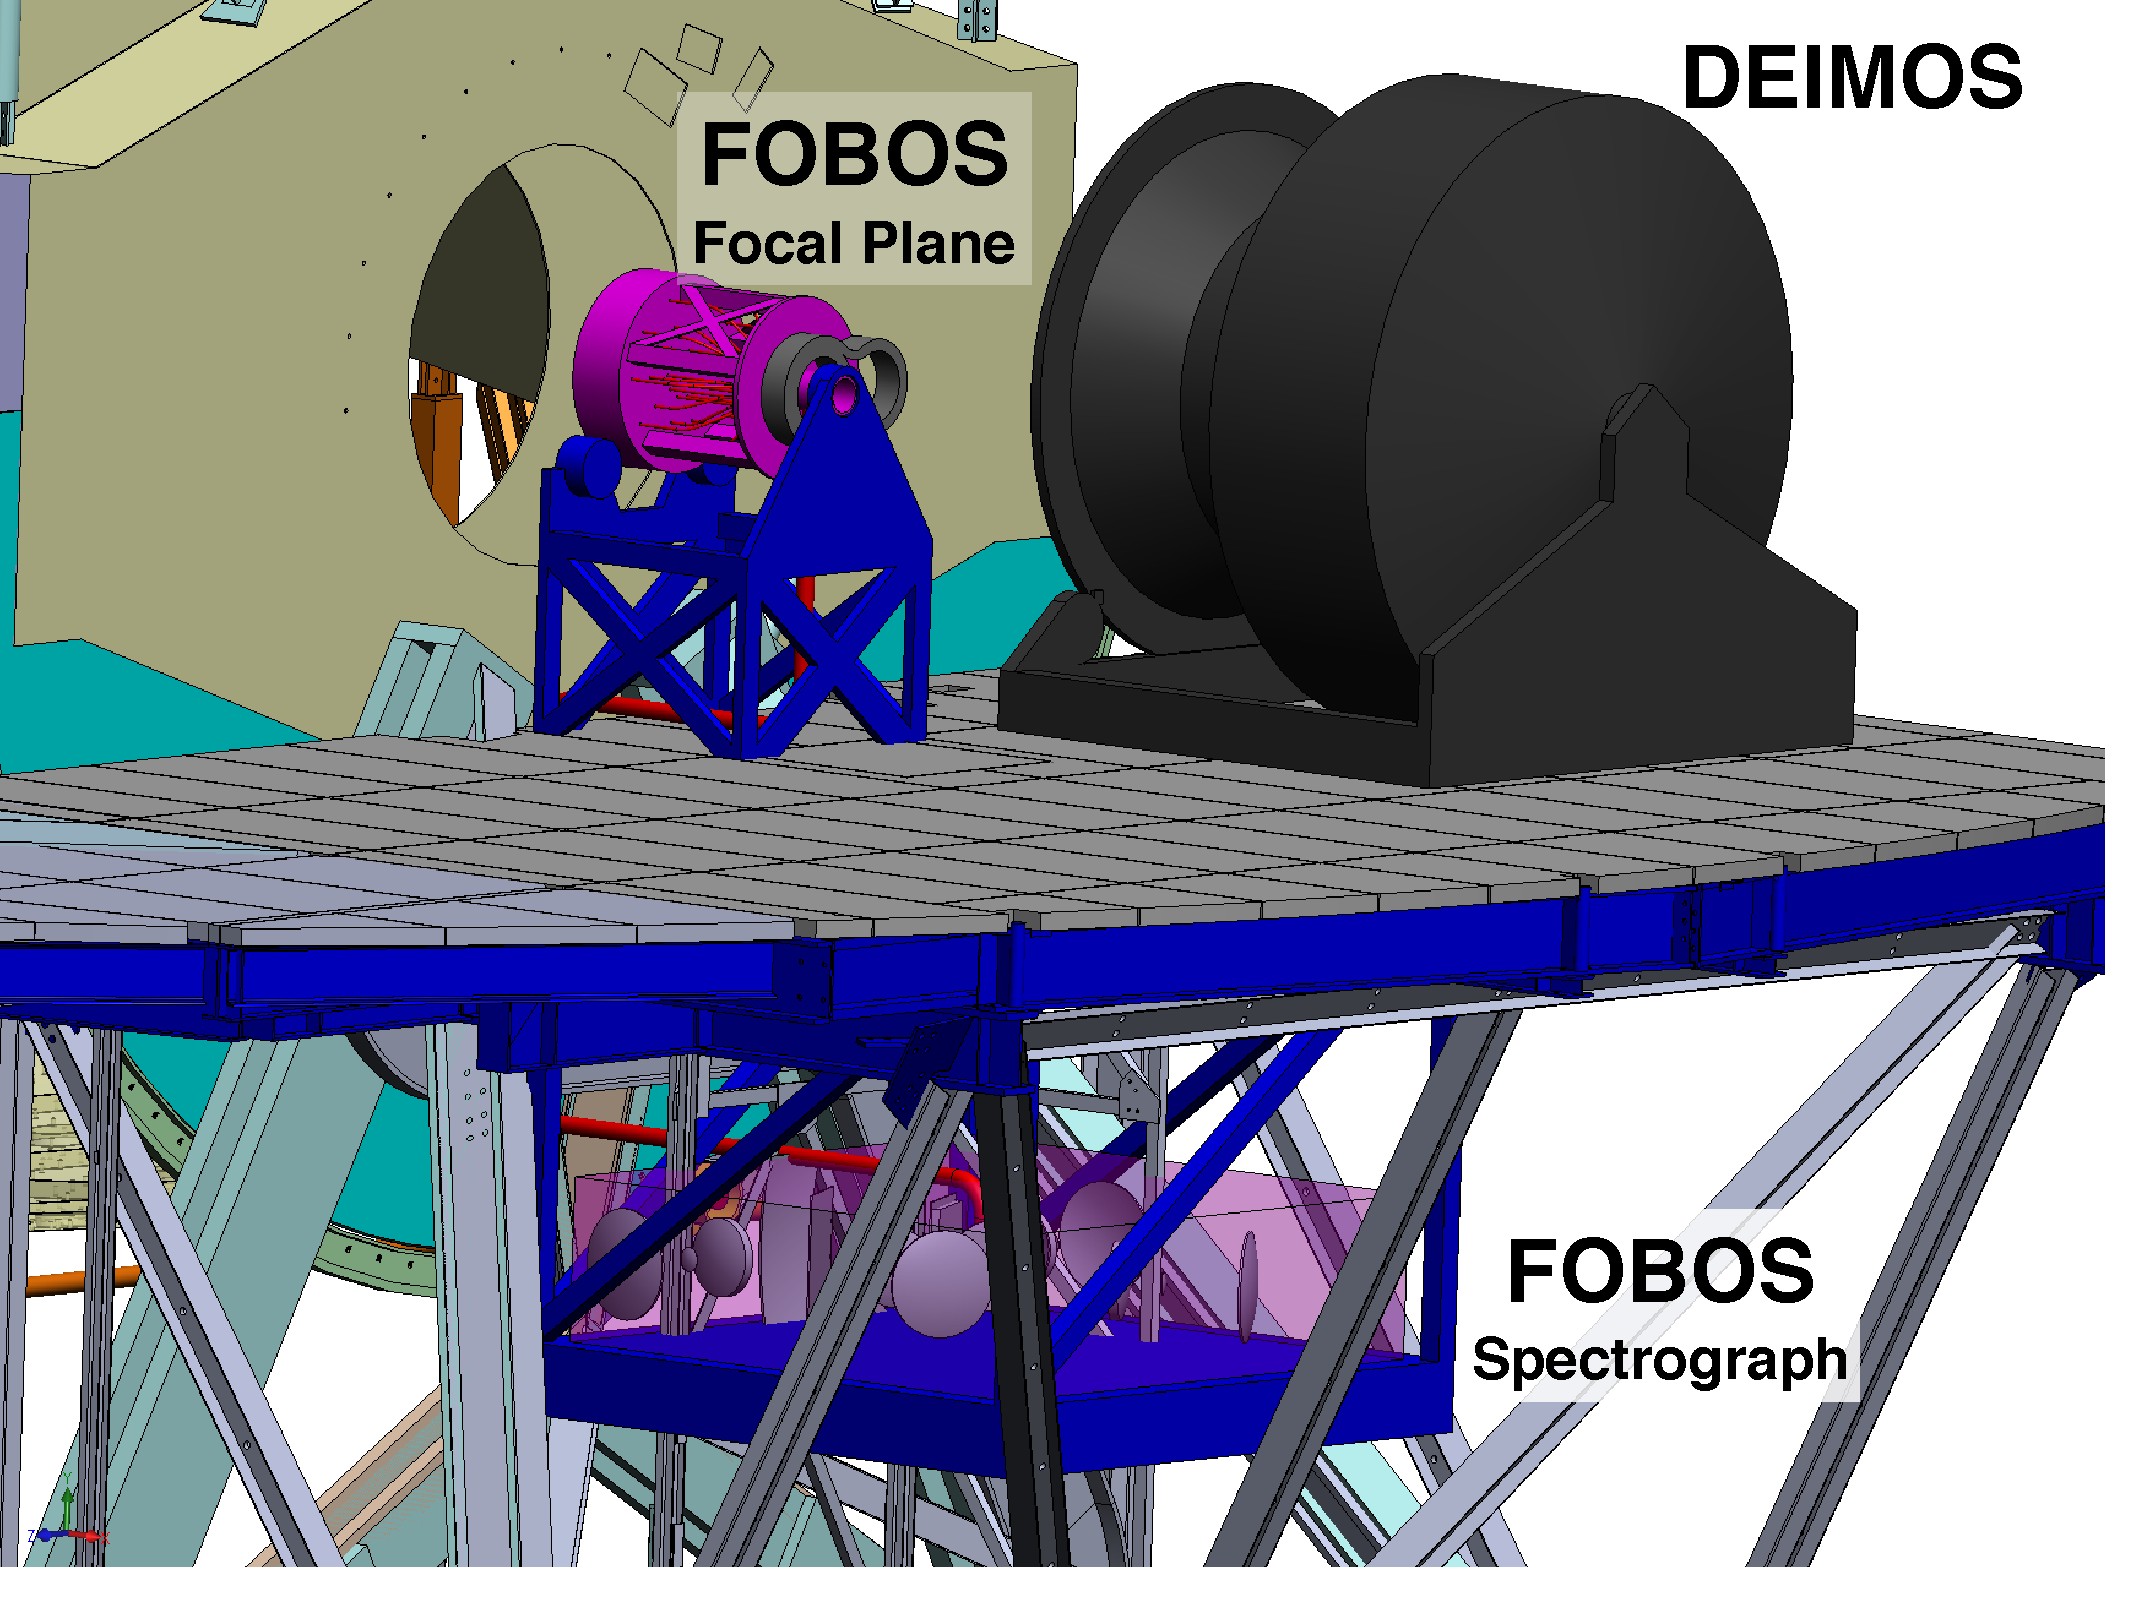
\includegraphics[width=0.6\textwidth, angle=0]{figs/FOBOSatKeck_v1.pdf}
%    \hspace{0.1cm} \vspace{2in}
%    \parbox[b]{0.3\textwidth}{\small {\bf Figure ??:} Rendering of FOBOS instrument systems deployed at the Keck II Nasmyth port.  By mounting the FOBOS spectrographs under the Nasmyth platform, other instruments like DEIMOS can maintain access to the telescope. \vspace{2cm}}}}

\begin{figure}[h!]
%
\vskip -0.1in
%
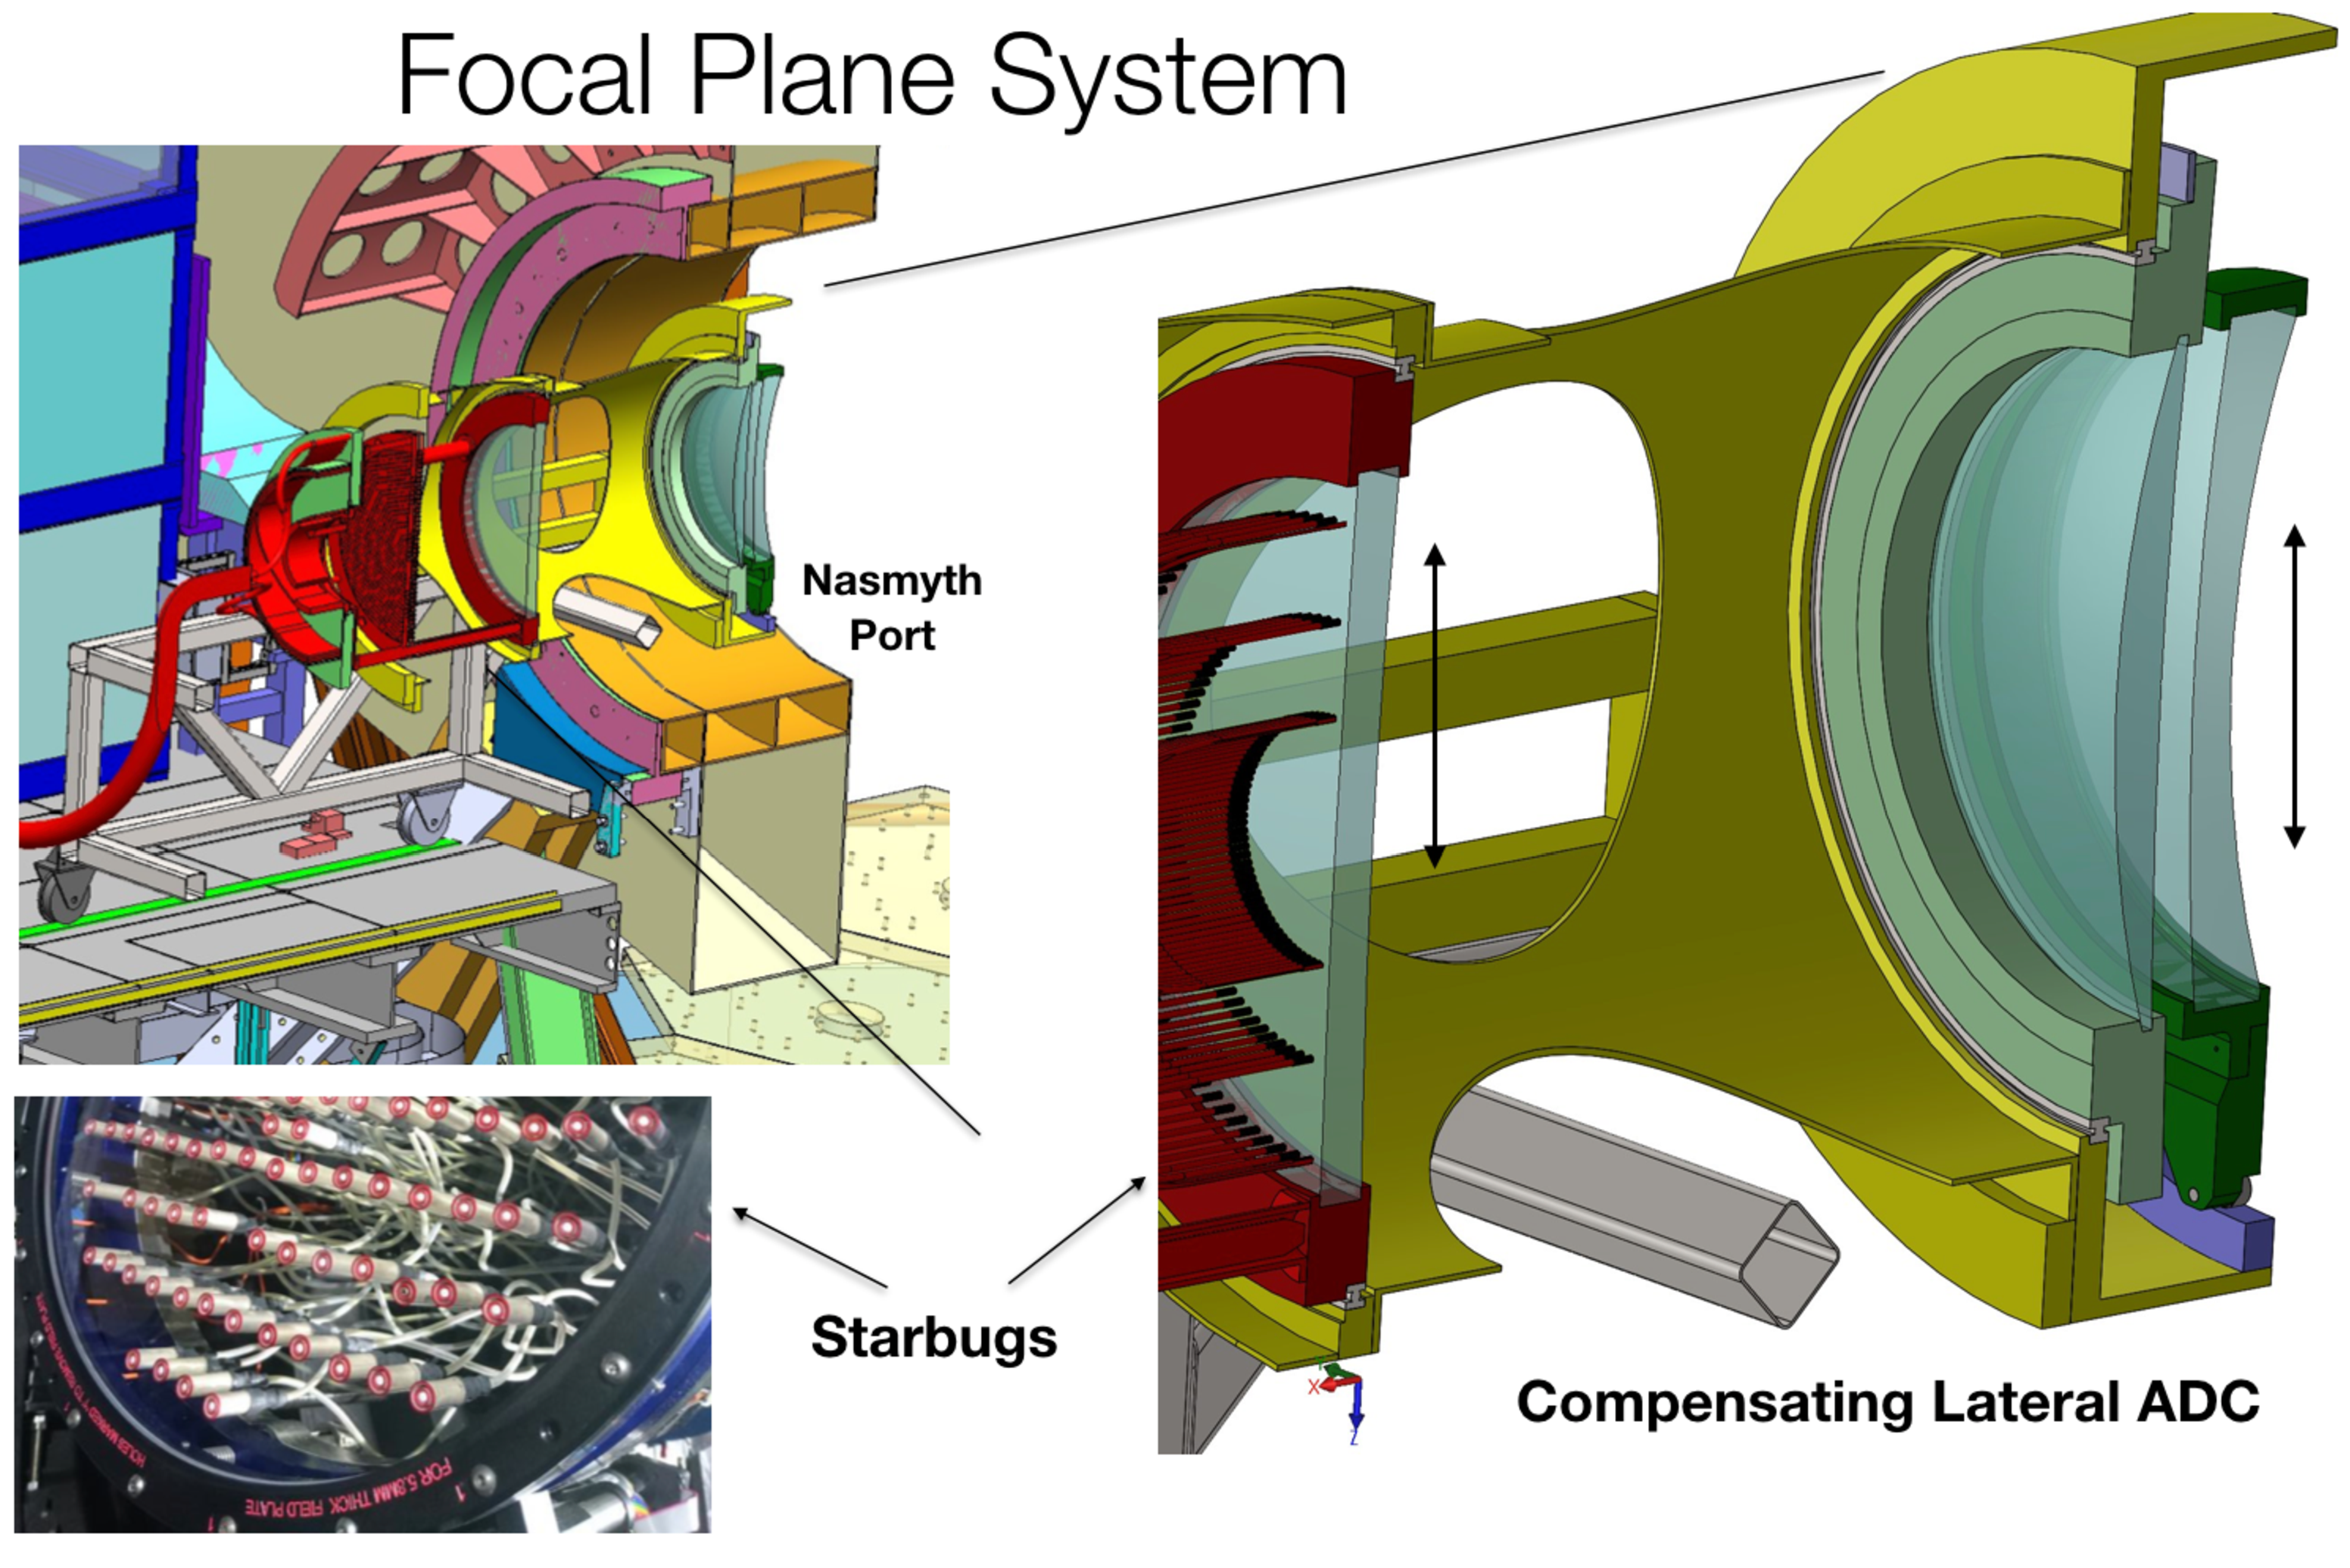
\includegraphics[width=\textwidth]{figs/FOBOS_FocalPlane.pdf}
%
\caption{\small {\it Left}: Rendering of FOBOS focal plane system
deployed at the Keck II Nasmyth port.  By mounting the FOBOS
spectrographs under the Nasmyth platform, other instruments like DEIMOS
can maintain access to the telescope. {\it Right}: Rendering of the ADC and focal surface with Starbugs mounted (red cylinders).  {\it Bottom-left}: Starbugs deployed on the TAIPAN instrument.}
%
\label{fig:focalplane}
%
\end{figure}

Mounted at the Nasmyth focus of Keck II Telescope at WMKO, FOBOS (Fig
\ref{fig:layout}) will be one of the most powerful spectroscopic
facilities deployed in the next decade.  FOBOS includes a compensating lateral
atmospheric dispersion corrector (CLADC, not pictured) to ensure that
target light from all wavelengths falls on allocated fibers while also
correcting image aberrations at the edges of the 20 arcmin diameter Keck
field.  Each of the CLADC lenses is 946 mm in diameter, the first two
closely spaced with lateral relative motions enabled by three
barrel-mounted actuators.  The final CLADC lens surface serves as the
vertical mounting plate for roaming Starbugs fiber positioners.  It
translates to track focal plane tilt.  Starbugs patrol a large on-sky
area ($\sim$1 arcmin), enabling flexible and dynamic targeting
configurations with adjacent fibers as close as 10 arcsec.

A total of 1800 150-$\mu$m core diameter fibers are deployed at the curved focal plane.  Fore-optics on the front end
of each fiber demagnify and speed up the beam (from f/15 to f/5) for better coupling to the fiber numerical aperture
and to minimize losses from focal ratio degradation.  The focal plane plate rotates and translates to follow image
positions as the telescope tracks across the sky.  The fiber run is kept at less than 10m to maintain high throughput
at UV wavelengths.  Special care is given to stress-relief cabling to minimize variable focal ratio degradation over
the fiber run.

Sets of 600 fibers feed each of three identical spectrographs (Fig
\ref{fig:layout}).  Each spectrograph uses a series of dichroics to
divide the 259 mm diameter collimated beam into four wavelength channels with combined, instantaneous
coverage from 0.31--1 $\mu$m.  Fused-silica etched (FSE) gratings provide mid-channel spectral resolutions of $R
\sim 3500$ at high diffraction efficiency in each channel.  The dispersed light is focused by an f/1.1
catadioptric camera\footnote{Based on the camera design for the Multi-Object Optical and Near-infrared Spectrograph (MOONS) on the Very Large Telescope (VLT).} and recorded by an on-axis 4k$\times$4k CCD mounted
at the center of the first camera lens element.  Spectrographs are
mounted in a temperature controlled housing installed under the Nasmyth
Deck to allow space for other Keck instruments above.  The end-to-end
instrument throughput peaks at 60\% and is greater than 30\% at all wavelengths
%\comment{compare to PEP}.

FOBOS includes observatory level systems for precise instrument
calibration using dome-interior screen illumination, a metrology system
for accurate fiber positioning, and guide cameras for field acquisition
and guiding.  The instrument design envisions future upgrades including
alternate collecting modes that deploy multiple fiber bundles, feeds to
other fiber-based spectrographs at different wavelengths or spectral
resolutions, and the ability to support and benefit from image
corrections with Ground-Layer Adaptive Optics.
